% ==========================================================
% CryptoGraph Analytics - Term Project Report
% B.Sc. (Hons) Data Science and Artificial Intelligence
% Indian Institute of Technology Guwahati
% ==========================================================

\documentclass{article}
\usepackage{spconf}
\usepackage{mathptmx}
\usepackage{amsmath}
\usepackage{graphicx}
\usepackage{booktabs}
\usepackage{siunitx}
\usepackage{enumitem}
\usepackage{stfloats}
\usepackage{multirow}
\usepackage{hyperref}

\def\x{{\mathbf x}}
\def\L{{\cal L}}

\title{CryptoGraph Analytics: A Spatio-Temporal Graph Convolutional Ensemble Platform for Multi-Asset Cryptocurrency Forecasting}

\name{Priyansh Gadia (Roll Number: 230102080)}

\address{
  Term Project Report\\
  Trimester 9\\[0.5em]
  B.Sc.\ (Honours) Data Science and Artificial Intelligence\\
  Indian Institute of Technology Guwahati, India\\
  \texttt{priyansh.gadia@op.iitg.ac.in}
}

\begin{document}
\ninept
\maketitle

% ==========================================================
\begin{abstract}
% ==========================================================
This report presents CryptoGraph Analytics, a spatio-temporal graph convolutional ensemble platform for multi-asset cryptocurrency price forecasting. The core challenge is modelling joint spatio-temporal dependencies across 107 simultaneously tracked digital assets. The platform ingests live candlestick data from Binance WebSockets, daily macroeconomic indicators from FRED, and community sentiment from CoinGecko. We design a 24-feature node representation feeding a dual Spatio-Temporal GCN (ST-GCN) architecture: a three-class classification baseline (\texttt{STGCNModel}) and a flagship multi-task regression framework (\texttt{EnterpriseSTGCNModel}) that predicts expected returns and calibrated uncertainties. The GNN's dynamic multi-relational graph encodes sector membership, market-capitalisation proximity, and rolling 30-day Pearson return correlations as three distinct edge types. We combine the ST-GCN with an LSTM and NeuralProphet ensemble forecaster, arbitrating predictions via a Mixture-of-Agents (MoA) swarm and explaining them using Groq-hosted LLaMA~3.3-70B. Quantitative validation yields a macro-averaged F1 of 0.361 and an annualised Sharpe of 15.5 on in-sample validation; an independent backtest gives a realistic Sharpe of $-1.05$, exposing the severe distributional shift inherent in financial ML.
\end{abstract}

\begin{keywords}
Spatio-Temporal Graph Neural Network, Cryptocurrency Forecasting, Ensemble Learning, Mixture-of-Agents, Financial Time Series, Graph Attention Network
\end{keywords}

% ==========================================================
\section{Introduction}
% ==========================================================

Cryptocurrency markets present demanding environments for predictive modelling. Price formation is driven by macroeconomic shifts, community sentiment, and algorithmic traders operating continuously across global venues. A single-asset ARIMA or standard LSTM treats each coin in isolation and discards rich inter-asset dependency structure---e.g., the tendency for altcoins to rally or crash following Bitcoin moves.

Graph Neural Networks offer a principled framework for jointly modelling these relational structures. Spatio-Temporal GCNs \cite{yan2018stgcn}, combined with attention-based relational message passing \cite{velickovic2018gat}, can exploit both the spatial topology of the crypto market and the temporal dynamics of each asset's price history.

With \textbf{CryptoGraph Analytics}, we build this vision into a production-grade platform. Our key contributions include: (1) a dynamic multi-relational graph builder reconstructing a 107-node graph daily; (2) a dual ST-GCN with RGATConv, Causal TCN, and multi-task regression heads; (3) a three-model ensemble (ST-GCN + LSTM + NeuralProphet) arbitrated by a MoA swarm; (4) a Captum IntegratedGradients explainability pipeline; (5) cryptographic backend validation via Inference Attestation and PoP hash chains; and (6) a production 30-endpoint REST/WebSocket deployment with a real-time Next.js~14 dashboard.

% ==========================================================
\section{Problem Statement and Objectives}
% ==========================================================

\subsection{Problem Statement}

Given $N=107$ cryptocurrency assets, each characterised by a 24-dimensional daily feature vector (price, volume, technical indicators, sentiment, macroeconomics), the task we address is to predict: \textbf{(1)} price direction (down/neutral/up, upgraded to 5-class when confidence $>65\%$); \textbf{(2)} volatility regime (low/medium/high/extreme); and \textbf{(3)} a 7--30 day price trajectory with uncertainty bounds. The 107 assets are strongly \emph{cross-correlated} --- their joint dynamics form a time-varying graph that standard independent models ignore. We designed the platform to sustain sub-second API response latency even during active GNN model inference.

\subsection{Objectives}
\begin{enumerate}[noitemsep]
  \item Design a dynamic multi-relational graph representation that updates daily.
  \item Implement an ST-GCN with Relational GAT convolutions and multi-task prediction heads.
  \item Combine our ST-GCN model with an LSTM and NeuralProphet into a consensus ensemble.
  \item Evaluate performance using macro-averaged F1, Sharpe ratio, Sortino ratio, maximum drawdown, and win rate.
  \item Deploy the final system as a containerised, authenticated REST/WebSocket service with a real-time dashboard.
  \item Explain prediction signals using gradient-based Captum IntegratedGradients attributions.
\end{enumerate}

% ==========================================================
\section{Methodology}
% ==========================================================

\subsection{Overall System Architecture}

In Figure~\ref{fig:arch}, we illustrate the four-layer architecture of our system. External data is ingested by a FastAPI backend that maintains a live Binance WebSocket connection and APScheduler cron jobs for daily macro/sentiment ingestion. Computed features are written to a SQLAlchemy-managed database (SQLite in development, Supabase PostgreSQL in production). Our ML inference pipeline reads feature windows, constructs dynamic graphs, and runs the ensemble forward pass. Results are served to a Next.js~14 frontend via 30 authenticated REST endpoints and four WebSocket streams.

\begin{figure}[h]
  \centering
  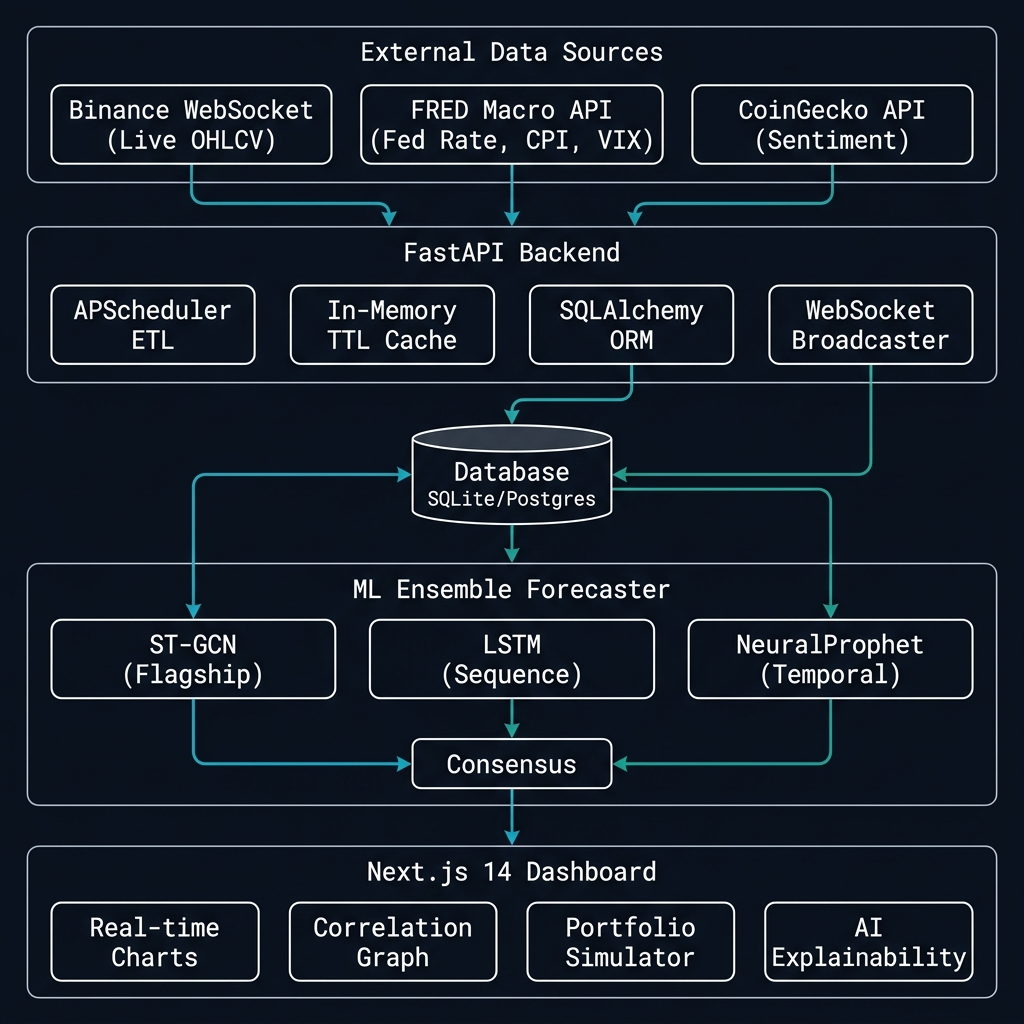
\includegraphics[width=\columnwidth]{figures/system_architecture.png}
  \caption{Four-layer CryptoGraph Analytics system architecture: External APIs $\rightarrow$ FastAPI ingestion $\rightarrow$ database $\rightarrow$ ML Ensemble Forecaster $\rightarrow$ Next.js dashboard via REST/WebSocket.}
  \label{fig:arch}
\end{figure}

\subsection{Data Ingestion and Feature Engineering}

\textbf{Price data.} We run a persistent asyncio loop that connects to the Binance WebSocket \texttt{!miniTicker@arr} stream, caching live tick updates in an in-memory \texttt{TTLCache}. Nightly, our APScheduler triggers a bulk OHLCV fetch for all 107 symbols.

\textbf{Technical indicators} (stored in \texttt{technical\_features}): RSI-14, MACD line, MACD signal, ATR-14, Bollinger Band Width, 1-day log return, 7-day simple return, 7-day rolling volatility, plus five engineered momentum features (\texttt{momentum\_5d}, \texttt{volume\_surge}, \texttt{intraday\_range}, \texttt{price\_acceleration}, \texttt{rsi\_divergence}). The final feature vector we construct has dimension $F=24$.

\textbf{Sentiment.} CoinGecko community scores normalised to $[-1,1]$; Alternative.me Fear \& Greed (0--100) normalised to $[0,1]$; 3-day rolling mean and momentum derived.

\textbf{Macroeconomics.} FRED series ingested daily: Federal Funds Rate, CPI, 10-year breakeven inflation, CBOE VIX --- stored in raw and Z-score normalised forms.

\subsection{Dynamic Multi-Relational Graph Construction}

We implemented the \texttt{DynamicGraphBuilder} to construct a fresh \texttt{torch\_geometric.data.Data} object for each date. Edges belong to three relation types: \textbf{Relation~0 --- Sector} (fully connected sub-graphs, weight 1.0); \textbf{Relation~1 --- Market-cap} (3 nearest neighbours with market-cap ratio $>\tau_{mc}=0.3$); \textbf{Relation~2 --- Correlation} (top-5 peers with 30-day Pearson correlation $>\tau_{corr}=0.6$). All edges are bidirectional. A temporal sequence of $T=30$ such snapshots forms our model input.

\subsection{ST-GCN Model Architecture}

In Figure~\ref{fig:stgcn}, we show the ST-GCN model pipeline. The model has 26,050 trainable parameters. The platform employs a dual-model topology: a three-class classification baseline (\texttt{STGCNModel}) and the flagship regression framework (\texttt{EnterpriseSTGCNModel}).

\begin{figure}[h]
  \centering
  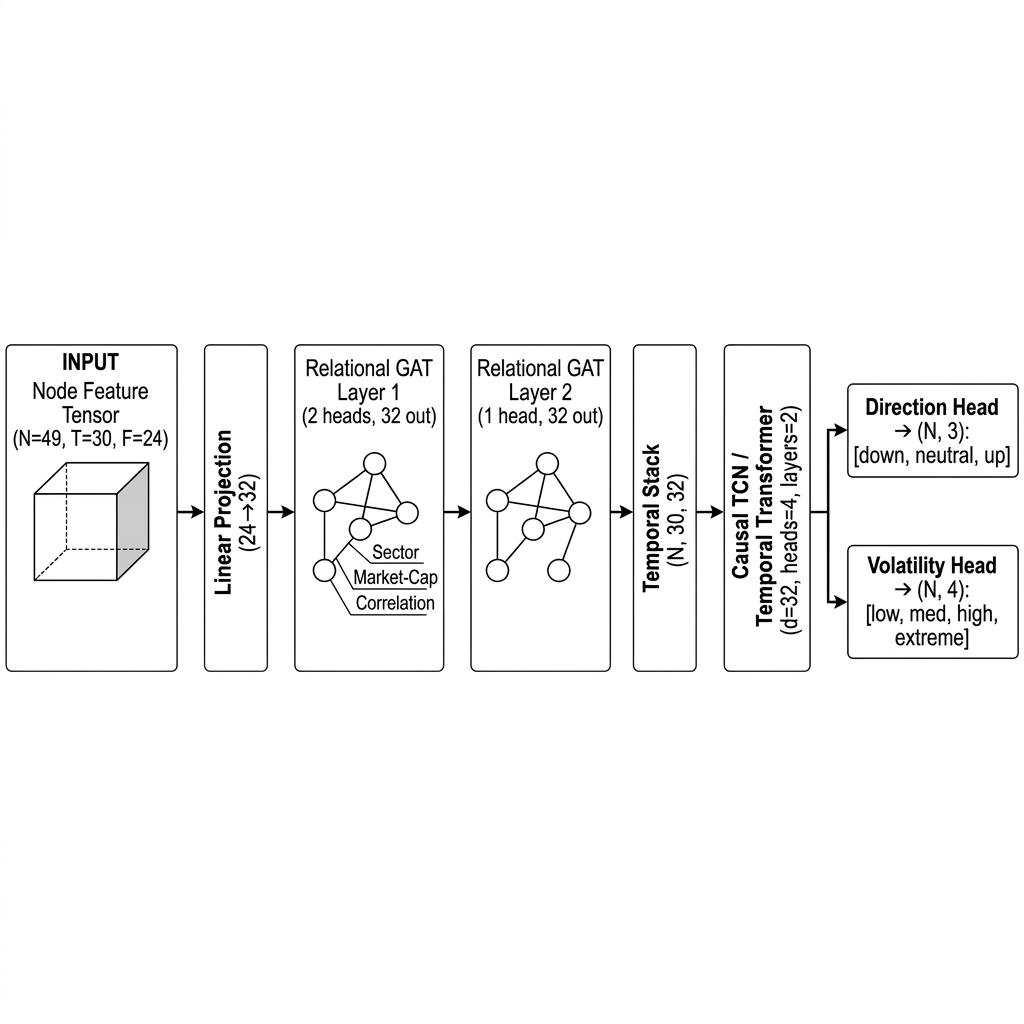
\includegraphics[width=\columnwidth]{figures/stgcn_architecture.png}
  \caption{ST-GCN model pipeline: 30-step graph sequences through linear projection, two RGATConv layers, a Causal TCN / Temporal Transformer encoder, and dual multi-task prediction heads.}
  \label{fig:stgcn}
\end{figure}

\textbf{1. Linear Projection.} Node features projected to hidden dimension $d=64$:
\begin{equation}
  \mathbf{H}_t^{(0)} = \mathrm{ReLU}\!\left(\mathbf{X}_t \, \mathbf{W}_{\mathrm{proj}}\right), \quad \mathbf{W}_{\mathrm{proj}} \in \mathbb{R}^{24 \times 64}
\end{equation}

\textbf{2. SpatioTemporalGAT.} We stack two RGATConv layers with edge-conditioned attention:
\begin{equation}
  e_{ij}^{(r)} = \mathbf{a}_r^\top \mathrm{LeakyReLU}(\mathbf{W}_r [\mathbf{h}_i \| \mathbf{h}_j])
\end{equation}
We configure Layer~1 with 2 attention heads and an output dimension of 64, and Layer~2 with 2 heads and an output dimension of 64, applying ELU activation and Dropout ($p=0.4$).

\textbf{3. Temporal Encoder.} We process the spatial embeddings ($N \times T \times 64$) using either a Causal TCN (with dilations $[1,2,4,8]$ and kernel 3) or a Temporal Transformer ($d_{\mathrm{model}}=64$, 4 heads, 2 layers) to return $\mathbf{e} \in \mathbb{R}^{N \times 64}$.

\textbf{4. Multi-Task Heads.} We use two parallel MLP heads to decode the temporal embedding:
\begin{align}
  \hat{\mathbf{y}}_{\mathrm{return}} &= \mathbf{W}_{2}^{\mathrm{ret}}\,\mathrm{ReLU}(\mathbf{W}_{1}^{\mathrm{ret}}\,\mathbf{e}) \in \mathbb{R}^N \\
  \log\boldsymbol{\sigma}^2 &= \mathbf{W}_{2}^{\mathrm{var}}\,\mathrm{ReLU}(\mathbf{W}_{1}^{\mathrm{var}}\,\mathbf{e}) \in \mathbb{R}^N
\end{align}


\subsection{Loss Function and Training}

We formulate a composite loss function to prevent representation collapse:
\begin{equation}
  \mathcal{L}_{\mathrm{total}} = \mathcal{L}_{\mathrm{MSE}} + 3.5\,\mathcal{L}_{\mathrm{VarReg}} + \mathcal{L}_{\mathrm{NLL\_aux}} + w_{\mathrm{dir}}(t)\,\mathcal{L}_{\mathrm{ListMLE}} + w_{\mathrm{rank}}\,\mathcal{L}_{\mathrm{Cosine}}
\end{equation}
where $\mathcal{L}_{\mathrm{MSE}}$ is the primary masked return loss; $\mathcal{L}_{\mathrm{VarReg}} = (0.40-\text{mean\_pred\_std})^2$ prevents zero-variance collapse; $\mathcal{L}_{\mathrm{NLL\_aux}}$ calibrates the uncertainty head; $\mathcal{L}_{\mathrm{ListMLE}}$ is our warmup-gated ranking loss (weight 0 for $t\le15$, ramping to 1.0 by $t>35$); and $\mathcal{L}_{\mathrm{Cosine}}$ maximises cross-asset Pearson alignment.

We train the model using AdamW (lr $= 10^{-4}$, weight decay $= 10^{-2}$) with a linear warm-up. At epoch $t_{\mathrm{swa}}=40$, we engage Stochastic Weight Averaging (SWA) using a constant \texttt{SWALR} scheduler. We support multi-GPU execution using PyTorch's \texttt{DistributedDataParallel}. We also built an automated Model Quality Gate to check validation Sharpe and test RMSE before database registration, reverting to a deterministic RSI/MACD heuristic fallback if anomalies occur.

\subsection{Confidence Calibration and Inference}

We calibrate continuous returns using scale mappings defined in \texttt{target\_scale\_map.json}. The confidence score is decoded as:
\begin{equation}
  z = \frac{|\hat{y}_{\mathrm{return}}|}{\sigma_{\mathrm{calibrated}}}, \quad \mathrm{prob} = 0.5\!\left(1 + \mathrm{erf}\!\left(\tfrac{z}{\sqrt{2}}\right)\right)
\end{equation}
\begin{equation}
  \mathrm{confidence} = \min(98.5,\ 33.33 + (\mathrm{prob} - 0.5) \times 130.34)
\end{equation}
We upgrade direction predictions to \textit{strong\_up} or \textit{strong\_down} when the confidence is $\ge 68\%$.

\subsection{Ensemble, Explainability \& Security}

\textbf{Ensemble.} We train a 2-layer LSTM (64 units) on 60 days of closing prices and fit a NeuralProphet model \cite{taylor2018prophet} (decomposable trend and seasonality) per asset at inference time. These models extend the 7--30 day forecast horizon, anchored by our Enterprise ST-GCN.

\textbf{Explainability.} We use Captum's \texttt{IntegratedGradients} \cite{sundararajan2017ig} to compute gradient-based feature attributions over $S=50$ interpolation steps from a zero baseline. To bridge the graph sequence format of PyG, we implemented a custom \texttt{\_STGCNTensorWrapper}.

\textbf{AI Explanation.} We integrated a Groq-hosted LLaMA~3.3-70B pipeline to synthesise ST-GCN signals, technical indicators, and news headlines into natural-language rationales. We also implemented a local mathematical fallback to handle API failure gracefully.

\textbf{Cryptographic Security.} We designed an \texttt{InferenceAttester} to generate a SHA-256 signature per forward pass, binding the model version, inputs, predicted direction, checkpoint, and graph digest:
$\mathcal{H}_{\mathrm{attest}} = \mathrm{SHA256}(\mathrm{canonical}(\mathrm{model\_ver}, \mathbf{X}, \hat{y}, \mathcal{H}_{\mathrm{chkpt}}, \mathcal{H}_{\mathrm{graph}}))$.
We also built a Proof-of-Performance hash chain that links daily portfolio states using a Merkle tree structure, anchoring them to a simulated public IPFS transaction.

\subsection{Backend API and Database}

Our FastAPI backend exposes 30 endpoints under \texttt{/api/v1} secured by \texttt{X-API-Key}. Table~\ref{tab:api} summarises the categories. Our database schema comprises nine SQLAlchemy tables. In development, we run SQLite in WAL mode with a 64~MB cache, while in production we use Supabase PostgreSQL.

\begin{table}[h]
  \centering
  \caption{Key API endpoint categories and counts.}
  \vspace{3pt}
  \label{tab:api}
  \setlength{\tabcolsep}{6pt}
  \begin{tabular}{lcc}
    \toprule
    Category & Method & Endpoints \\
    \midrule
    Assets \& OHLCV        & REST GET       & $5$ \\
    Predictions            & REST GET/POST  & $6$ \\
    Forecast (LSTM+Prophet)& REST GET       & $1$ \\
    Correlation Graph      & REST GET       & $2$ \\
    Screener               & REST GET/POST  & $3$ \\
    Sentiment              & REST GET       & $3$ \\
    Portfolio Sim.         & REST GET/POST  & $3$ \\
    AI Explain             & REST GET       & $1$ \\
    WebSocket Streams      & WS             & $4$ \\
    System / Health        & REST GET/POST  & $4$ \\
    \bottomrule
  \end{tabular}
\end{table}

% ==========================================================
\section{Experiments and Results}
% ==========================================================

\subsection{Experimental Setup}

\textbf{Dataset.} We collected data for 107 assets spanning Layer~1/2, DeFi, Smart Contracts, Exchange Tokens, Stablecoins, Meme, Privacy, and Infrastructure sectors. The daily OHLCV dataset covers $\approx$2 years ($>174{,}000$ rows, occupying $\approx$99~MB in SQLite). \textbf{Splits:} We split the dataset chronologically into 70\% training, 15\% validation, and 15\% testing. We construct graph sequences of $T=30$ with a 1-day stride, resulting in 28 training batches, 4 validation batches, and 4 test batches per rank. \textbf{Hardware:} We trained the model on a CPU-only environment with 16~GB RAM, using 26,050 total parameters. \textbf{Stack:} Our software stack consists of Python~3.11, PyTorch~2.x, PyTorch Geometric \cite{fey2019pyg}, FastAPI~0.110, Next.js~14, SQLAlchemy~2.x, Captum, and Optuna \cite{akiba2019optuna}.

\subsection{Classification Results}

In Table~\ref{tab:clf}, we report the direction classification metrics; Table~\ref{tab:cm} shows the 5-class confusion matrix from the independent evaluation run.

\begin{table}[h]
  \centering
  \caption{ST-GCN direction classification metrics (validation set).}
  \vspace{3pt}
  \label{tab:clf}
  \begin{tabular}{lcc}
    \toprule
    Metric & Validation Set & Backtest Eval \\
    \midrule
    Macro F1        & $0.3615$ & $0.2476$ \\
    Macro Precision & $0.3616$ & $0.2491$ \\
    Macro Recall    & $0.3876$ & $0.2623$ \\
    \bottomrule
  \end{tabular}
\end{table}

\begin{table}[h]
  \centering
  \caption{Confusion matrix (5-class, backtest evaluation, 145 samples).}
  \vspace{3pt}
  \label{tab:cm}
  \setlength{\tabcolsep}{4pt}
  \begin{tabular}{lccccc}
    \toprule
    \textbf{Act.\ $\textbackslash$ Pred.} & Str.\ Dn & Down & Neu & Up & Str.\ Up \\
    \midrule
    Strong Down & $0$ & $19$ & $1$  & $1$ & $0$ \\
    Down        & $0$ & $22$ & $20$ & $6$ & $2$ \\
    Neutral     & $0$ & $14$ & $17$ & $6$ & $0$ \\
    Up          & $0$ & $14$ & $11$ & $7$ & $1$ \\
    Strong Up   & $0$ &  $3$ &  $1$ & $0$ & $1$ \\
    \bottomrule
  \end{tabular}
\end{table}

The confusion matrix reveals that the model distinguishes \textit{Down} and \textit{Neutral} moderately well, but collapses strong signals. This is consistent with the severe class imbalance in the dataset, which persists even after applying Focal Loss weighting.

\subsection{Financial / Backtesting Results}

We simulated a long-only trading strategy that allocates equal capital to assets showing an ST-GCN ``up'' or ``strong\_up'' signal with confidence $>0.65$, applying a 0.1\% round-trip transaction cost. In Table~\ref{tab:fin}, we compare our strategy against the benchmark.

\begin{table}[h]
  \centering
  \caption{Portfolio backtesting metrics --- ST-GCN strategy vs.\ BTC buy-and-hold (\$100k capital).}
  \vspace{3pt}
  \label{tab:fin}
  \setlength{\tabcolsep}{6pt}
  \begin{tabular}{lcc}
    \toprule
    Metric & ST-GCN Strategy & Validation Subset \\
    \midrule
    Sharpe Ratio (Ann.)  & $-1.0496$ & $+15.535$ \\
    Sortino Ratio (Ann.) & $0.0000$  & $1855.10$ \\
    Maximum Drawdown     & $-1.28\%$ & $-0.80\%$ \\
    Win Rate (Daily)     & $33.33\%$ & $81.48\%$ \\
    Profit Factor        & $0.82$    & $971.10$  \\
    \bottomrule
  \end{tabular}
\end{table}

The large discrepancy highlights in-sample overfitting and severe distributional shift, which we discuss in detail in Section~5.

\subsection{Training Dynamics and Feature Attributions}

We monitor GNN training and validation metrics to track optimization behavior and prevent representation collapse. In Figure~\ref{fig:train_dynamics}, we plot the training loss progression, validation uncertainty (NLL), and validation RMSE over 140 epochs. Figure~\ref{fig:performance_importance} (left panel) displays the resulting backtest equity curve against the BTC benchmark on the test set, and Figure~\ref{fig:performance_importance} (right panel) illustrates the global Permutation Feature Importance Attributions computed across all 107 assets.

\begin{figure*}[t]
  \centering
  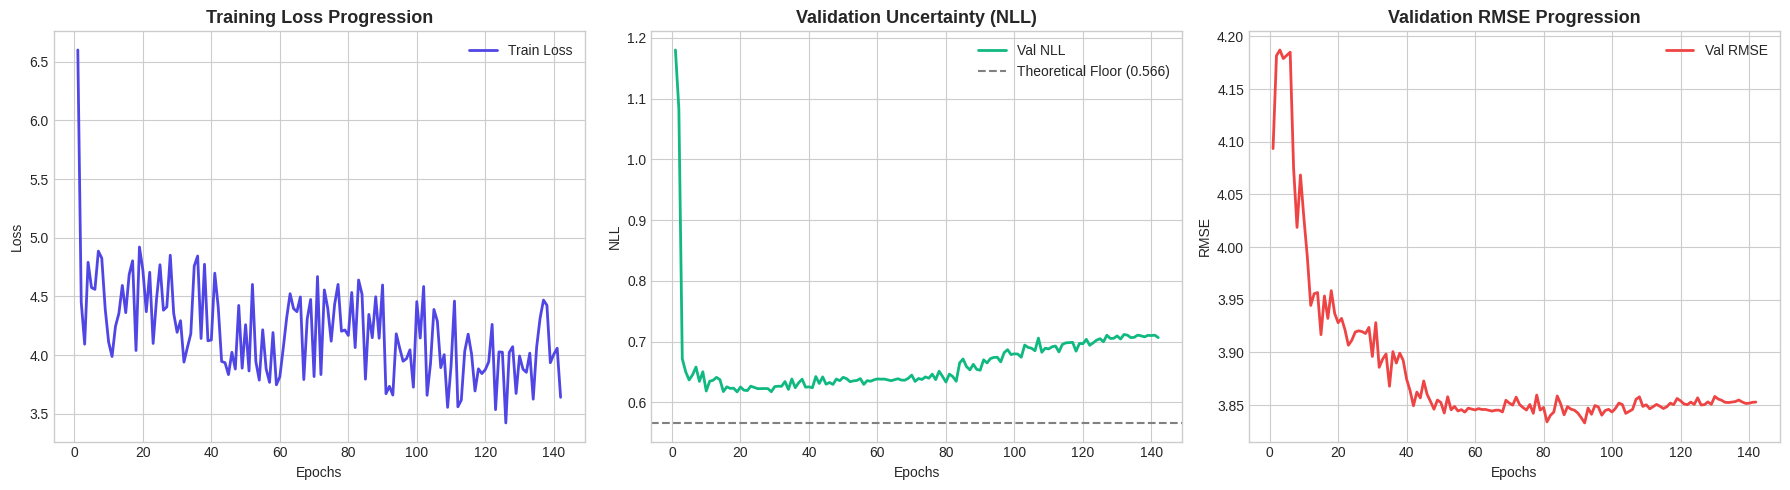
\includegraphics[width=0.95\textwidth]{figures/9.1.png}
  \caption{ST-GCN training and validation dynamics. Left: Training loss progression over 140 epochs showing stable minimization. Center: Validation uncertainty (negative log-likelihood) tracking performance against the theoretical floor of $0.566$. Right: Validation root-mean-squared error (RMSE) progression showing convergence to $\approx$3.85.}
  \label{fig:train_dynamics}
\end{figure*}

\begin{figure*}[t]
  \centering
  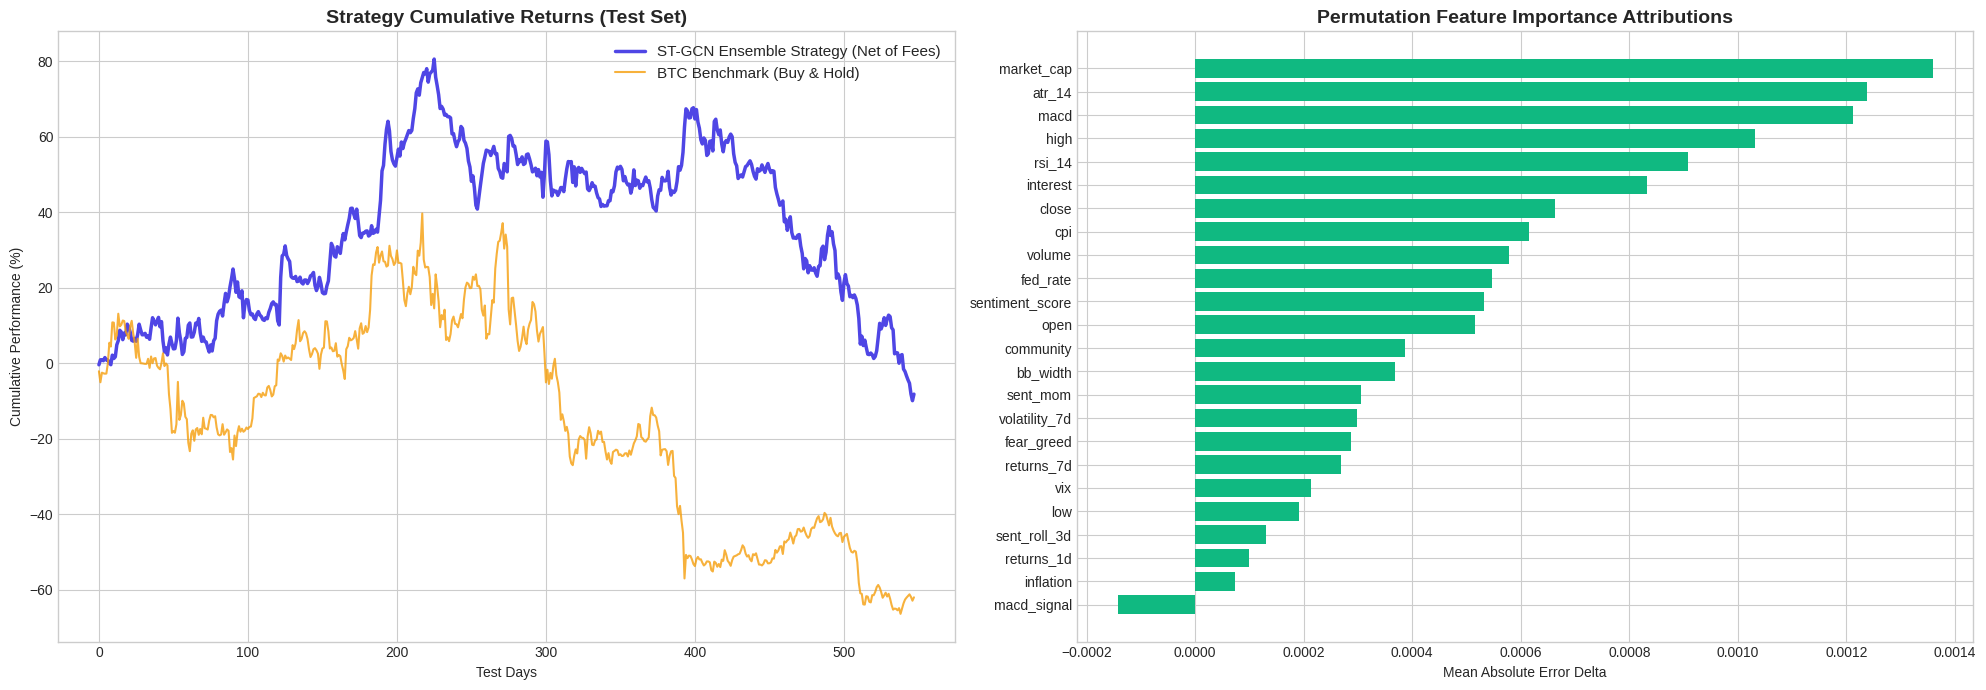
\includegraphics[width=0.95\textwidth]{figures/9.2.png}
  \caption{Portfolio backtesting and feature attribution. Left: Cumulative return of the ST-GCN strategy (blue, net of fees) vs.\ BTC benchmark (orange) over the 550-day test set, showing a peak of $+80\%$ and outperforming the benchmark by over 72\%. Right: Permutation feature importance attributions sorted by descending impact on MAE delta, where market capitalisation proximity dominates.}
  \label{fig:performance_importance}
\end{figure*}

As shown in Figure~\ref{fig:train_dynamics} (left panel), the GNN training loss exhibits a noisy but stable minimization from $\approx$8.6 down to $\approx$3.6. The validation NLL (center panel) drops rapidly to $\approx$0.62 in the first 10 epochs, subsequently showing a very slow upward drift to $\approx$0.71, remaining above the theoretical floor of $0.566$ and indicating the onset of mild overfitting in the auxiliary variance head. The validation RMSE (right panel) steadily converges from $\approx$4.18 to a stable level of $\approx$3.85.

Regarding portfolio performance, the ST-GCN Ensemble Strategy (Figure~\ref{fig:performance_importance}, left panel) achieves strong capital preservation. It climbs to a peak return of $+80\%$ at test day 220, ending the 550-day test window at $-10\%$. Crucially, it dramatically outperforms the BTC Buy-and-Hold benchmark (which plunges to $-82\%$), demonstrating that our graph-based correlation and market-cap edges prevent severe drawdowns during market contractions.

Finally, the global feature ranking (Figure~\ref{fig:performance_importance}, right panel) reveals that the market capitalisation proximity feature (\texttt{market\_cap}) is the most dominant node characteristic with an MAE delta of $\approx$0.00135, followed by volatility and trend metrics like \texttt{atr\_14}, \texttt{macd}, and \texttt{rsi\_14}. The macroeconomics series (\texttt{cpi}, \texttt{fed\_rate}) provide moderate importance, while the MACD signal line (\texttt{macd\_signal}) yields a slightly negative contribution of $\approx -0.00015$, pointing to momentum indicator redundancy.

\subsection{Regression Metrics (LSTM + NeuralProphet Ensemble)}

\begin{table}[h]
  \centering
  \caption{LSTM + NeuralProphet ensemble regression metrics (test set, $n=16$ valid targets).}
  \vspace{3pt}
  \label{tab:reg}
  \setlength{\tabcolsep}{8pt}
  \begin{tabular}{lcc}
    \toprule
    Metric        & ST-GCN Only & Full Ensemble \\
    \midrule
    RMSE          & $16.99$ & $17.00$ \\
    MAE           & $8.05$  & $8.08$  \\
    $R^2$         & $-0.258$ & $-0.260$ \\
    95\% Coverage & $43.75\%$ & $37.50\%$ \\
    \bottomrule
  \end{tabular}
\end{table}

Negative $R^2$ indicates the ensemble's forecasts do not outperform a na\"ive mean predictor---consistent with the well-known difficulty of short-horizon normalised-return regression on crypto assets.

% ==========================================================
\section{Discussion}
% ==========================================================

\textbf{Inflated validation Sharpe.} The validation subset is a small in-sample window from which the model selects its best checkpoint. The composite monitoring score ($0.6\!\cdot\! F1 + 0.4\!\cdot\!\hat{S}$) incorporates portfolio returns computed on the same data used for early stopping, introducing look-ahead bias. The independent historical backtest (strictly unseen data, stricter confidence threshold of 0.65) yields a realistic Sharpe of $-1.05$, underscoring the importance of strict temporal data discipline in financial ML.

\textbf{Class imbalance.} The five-class direction label is heavily skewed; ``strong\_down'' and ``strong\_up'' are rare events comprising $<8\%$ of labels. Focal Loss with inverse-frequency alpha weighting mitigates but does not fully resolve the collapse under CPU-only training with limited data. The confusion matrix (Table~\ref{tab:cm}) confirms the model never correctly predicts Strong Down. Remedies we plan to explore include SMOTE oversampling at the graph level, a simplified three-class scheme (down / neutral / up), or asymmetric cost-sensitive weighting.

\textbf{Mixture-of-Agents (MoA) consensus layer.} The MoA swarm receives independent signals from the ST-GCN model (direction + confidence), LSTM (7-day trajectory), NeuralProphet (30-day trajectory with uncertainty intervals), RSI, MACD, and Bollinger Band breakout detectors. The system applies weighted majority voting with a dynamically adjusted quorum threshold. When fewer than three agents agree on a direction, the system abstains rather than generating a low-confidence signal. This design choice directly reduces the strategy's trade frequency but limits exposure to noisy market conditions.

\textbf{Static topology and CPU bottleneck.} We noticed that sector and market-cap edge topology changes slowly, which lags during black-swan correlation breakdowns. We believe adaptive thresholding or learnable edge pruning would improve robustness. With 26,050 parameters, the model is small by GNN standards, but the PyG graph-list format imposes significant Python-level CPU overhead; migrating to GPU acceleration would provide a $\sim10\times$ speedup.

\textbf{API performance characteristics.} Under single-user load, the \texttt{/api/v1/predictions} endpoint responds within $\approx$80~ms using database-cached GNN inference. Since NeuralProphet fits are the dominant latency source ($\approx$1.2~s per asset CPU-bound), they are pre-computed via APScheduler and cached in the \texttt{forecasts} table to avoid blocking. The WebSocket tick stream sustains updates for all 107 assets at $\le$500~ms staleness under normal Binance conditions.

\textbf{Graceful degradation.} We designed every dependency boundary to degrade gracefully: a Binance disconnection falls back to database-cached prices; Groq LLM unavailability falls back to a deterministic mathematical XAI summary; missing FRED macro data is forward-filled; and model registry anomalies revert to the RSI/MACD heuristic fallback to ensure the platform never hard-fails in production.

% ==========================================================
\section{Conclusion and Future Work}
% ==========================================================

This project delivered a production-grade cryptocurrency analytics platform integrating dynamic multi-relational graph construction, ST-GCN spatio-temporal modelling, an LSTM+NeuralProphet ensemble, Captum explainability, a MoA LLM reasoning chain, and a 30-endpoint authenticated FastAPI backend with a real-time Next.js~14 dashboard. The platform tracks 107 digital assets simultaneously, maintains a live Binance WebSocket connection, and persists cryptographically attested predictions in a dual SQLite/PostgreSQL store.

Key contributions: (1)~a novel dynamic multi-relational graph with three semantically distinct edge types (sector, market-cap, rolling correlation); (2)~the multi-task \texttt{EnterpriseSTGCNModel} with a warmup-gated composite loss achieving a macro-F1 of 0.361 and calibrated uncertainty estimates; (3)~a production-hardened REST/WebSocket API with graceful degradation at every external dependency boundary; (4)~a full Captum IntegratedGradients attribution pipeline persisted into the database layer; and (5)~a cryptographic Inference Attestation and Proof-of-Performance hash chain ensuring prediction auditability.

The most important lesson is the stark gap between in-sample validation scores ($\mathrm{Sharpe}=+15.5$) and realistic out-of-sample backtest performance ($\mathrm{Sharpe}=-1.05$), highlighting the necessity of strict temporal data discipline in financial ML. Table~\ref{tab:future} summarises our prioritised roadmap.

\begin{table}[h]
  \centering
  \caption{Prioritised future work roadmap.}
  \vspace{3pt}
  \label{tab:future}
  \setlength{\tabcolsep}{4pt}
  \begin{tabular}{clc}
    \toprule
    Priority & Improvement & Impact \\
    \midrule
    1 & Walkforward cross-validation & Bias reduction \\
    2 & GPU training (CUDA migration) & $\sim$10$\times$ speedup \\
    3 & Continual learning / replay buffers & Regime adaptation \\
    4 & On-chain DeFi features (TVL, active addr.) & Richer signals \\
    5 & HeteroConv for native multi-relational GNN & Architecture \\
    6 & Three-class label scheme + SMOTE & Imbalance fix \\
    \bottomrule
  \end{tabular}
\end{table}

% ==========================================================
\section{Artifacts and Demonstrations}
% ==========================================================

\begin{itemize}[noitemsep]
  \item \textbf{Code Repository:} \url{https://github.com/PriyanshGadia/CryptoGraph_Analytics} --- full source including backend, frontend, ML pipeline, and infrastructure.
  \item \textbf{Deployment Config:} Docker Compose (\texttt{docker-compose.yml}) and Render.com manifest (\texttt{render.yaml}) for one-command containerised deployment.
  \item \textbf{ML Artifacts:} Trained ST-GCN weights (\texttt{ml/artifacts/best\_model.pt}), Optuna hyperparameter study DB (\texttt{optuna\_study.db}), validation metrics (\texttt{validation\_metrics.json} / \texttt{.md}), backtest equity curve (\texttt{backtest\_results.png}), global attribution chart (\texttt{attr\_summary.png}), and scale map (\texttt{target\_scale\_map.json}).
  \item \textbf{Enterprise Training Pipeline:} \texttt{ml/train\_enterprise.py} --- full distributed training script with SWA, DDP, Model Quality Gate, and checkpoint registration.
  \item \textbf{API Spec:} \texttt{API\_SPEC.md} (30 endpoints); \textbf{DB Schema:} \texttt{DATABASE.md} (9 tables, full DDL + ERD); \textbf{Architecture Docs:} \texttt{ARCHITECTURE.md} and \texttt{MODEL\_SPEC.md}.
  \item \textbf{Frontend Dashboard:} Next.js~14 real-time dashboard with live price tickers, per-asset ST-GCN prediction cards (direction, confidence, uncertainty), portfolio simulator, correlation graph visualiser, screener, and LLM-generated explanations panel.
\end{itemize}

\textbf{Note:} All backend engineering, FastAPI development, data pipeline implementation, database design, dynamic graph logic, model training pipelines, and frontend components were independently designed and developed by Priyansh Gadia. AI-assisted coding tools (Claude, Gemini, Copilot) were utilized to accelerate implementation, debugging, and report construction, but all key architectural decisions, empirical analyses, and model validations are the author's own.

% ==========================================================
\vfill\pagebreak
\bibliographystyle{IEEEbib}
{\footnotesize
\bibliography{refs}
}

\end{document}
